%% Slides for ".NET Programming" by Chunyu Wang <chunyu@hit.edu.cn> %%

\section{集合}

\begin{frame}
\frametitle{集合 System.Collections}

\begin{itemize}
\setlength{\itemsep}{8pt plus 1pt}
\item 集合,即一组对象 (\textit{object})
\item .NET 提供了 Lists, Stacks, Queues, Hash Tables 等集合结构
\item 提供了对集合操作的接口,如枚举器、迭代器
\item System.Collections.Generic 提供了相应的泛型结构
\end{itemize}

\end{frame}

\begin{frame}[fragile]
\frametitle{ArrayList}
\begin{lstlisting}
using System;
using System.Collections;
public class SamplesArrayList  {
  public static void Main()  {

    ArrayList myAL = new ArrayList();
    myAL.Add("Hello");
    myAL.Add("World");
    myAL.Add("!");

    Console.WriteLine("Count:    {0}", myAL.Count);
    Console.WriteLine("Capacity: {0}", myAL.Capacity);
    foreach ( Object obj in myAL )
      Console.Write( "{0} ", obj );
  }
}
\end{lstlisting}
\end{frame}

\begin{frame}[fragile]
\frametitle{Stack}
\begin{lstlisting}
using System;
using System.Collections;
public class SamplesStack  {
  public static void Main()  {

    Stack myStack = new Stack();
    myStack.Push("Hello");
    myStack.Push("World!");
    myStack.Pop();

    Console.WriteLine( "Count: {0}", myStack.Count );
    Console.Write( "Values:" );
    foreach ( Object obj in myStack )
      Console.Write( " {0}", obj );
  }
}
\end{lstlisting}
\end{frame}

\begin{frame}
\frametitle{ICollection 接口}
ICollection 继承了 IEnumerable,提供了基本的集合操作。
\begin{itemize}
\setlength{\itemsep}{8pt plus 1pt}
\item 特性
\begin{itemize}
\setlength{\itemsep}{6pt plus 1pt}
\item \texttt{int Count \{get;\} --- 当前集合中元素个数}
\item \texttt{object SyncRoot \{get;\} --- 用于多线程的同步}
\end{itemize}
\item 方法
\begin{itemize}
\item \texttt{void CopyTo(Array target, int startIdx)}
\end{itemize}
\end{itemize}
\end{frame}

\begin{frame}[fragile]
\frametitle{IList 接口}
IList 接口继承了 ICollection,提供了基于索引的操作方式。
\begin{itemize}
\item 索引器: \texttt{object this[int idx] \{ get; set; \}}
\begin{lstlisting}
ArrayList myAL = new ArrayList();
myAL[0] = "Hello"; myAL[1] = 123;
\end{lstlisting}
\item 特性
\begin{itemize}
\item \texttt{bool IsFixedSize \{ get; \}}
\item \texttt{bool IsReadOnly \{ get; \}}
\end{itemize}
\item 方法
\begin{itemize}
\item \texttt{int Add(object obj)} --- 添加元素
\item \texttt{void Clear()} --- 删除所有元素
\item \texttt{void Remove(object obj)} --- 删除第一个 \texttt{obj}
\item \texttt{Contains, IndexOf, Insert, RemoveAt}
\end{itemize}
\end{itemize}
\end{frame}

\begin{frame}
\frametitle{IDictionary 接口}
\CJKindent IDictionary 接口继承了 ICollection,提供了基于键 (\textit{key}) 的索引方式。
\begin{itemize}
\item 索引器:
  \begin{itemize}
  \item \texttt{object this[object key] \{ get; set; \}}
  \end{itemize}
\item 特性
\begin{itemize}
\item \texttt{bool IsFixedSize \{ get; \}}
\item \texttt{bool IsReadOnly \{ get; \}}
\item \texttt{ICollection Keys \{ get; \}} --- 返回所有键
\item \texttt{ICollection Values \{ get; \}} --- 返回所有值
\end{itemize}
\item 方法
\begin{itemize}
\item \texttt{void Add(object k, object v)}
\item \texttt{Clear, Contains, Remove, ...}
\end{itemize}
\end{itemize}
\end{frame}

\begin{frame}
\frametitle{ArrayList 类}
ArrayList 实现了 ICollection, IList, IEnumerable, ICloneable 接口。
\begin{itemize}
\item 构造函数
\begin{itemize}
\item \texttt{public ArrayList()}
\item \texttt{public ArrayList(ICollection c)}
\item \texttt{public ArrayList(int \textit{capacity})}
\end{itemize}
\item 特性
  \begin{itemize}
  \item \texttt{public virtual int Capacity \{ get; set; \}}
  \end{itemize}
\item 方法
  \begin{itemize}
  \item \texttt{public virtual void Sort()}
  \item \texttt{public virtual void Sort(IComparer \textit{comp})}
  \item \href{http://msdn2.microsoft.com/en-us/library/system.collections.arraylist_members.aspx}{\beamergotobutton{参考 MSDN}}
  \end{itemize}
\end{itemize}
\end{frame}

\begin{frame}
\frametitle{Hashtable 类}

\CJKindent Hashtable 使用 \textit{Hashing} 技术存储数据。将键转换
为\textit{Hash code},用于数据的索引,决定数据的存储位置。

\begin{itemize}
\item 键转换为 Hash code 的过程是自动的
\item 访问时也只需使用键本身,不使用 Hash code
\item 使用 Hashtable 可以提高字典的访问效率
\end{itemize}

\CJKindent Hashtable 实现了 IDictionary, ICollection, IEnumerable,
ISerializable, IDeserializationCallback, 和ICloneable 接口。
\end{frame}

\begin{frame}
\frametitle{Hashtable 的成员}
\begin{itemize}
\item 构造函数
\begin{itemize}
\item \small \texttt{public Hashtable()}
\item \small \texttt{public Hashtable(IDictionary c)}
\item \small \texttt{public Hashtable(int capacity)}
\item \small \texttt{public Hashtable(int capacity, float fillRatio)}
\end{itemize}
\item 特性
\begin{itemize}
\item \small \texttt{public virtual ICollection Keys \{ get; \}}
\item \small \texttt{public virtual ICollection Values \{ get; \}}
\end{itemize}
\item 方法
\begin{itemize}
\item \texttt{public virtual bool ContainsKey(object k)}
\item \texttt{public virtual bool ContainsValue(object v)}
\item \dots
\end{itemize}
\end{itemize}

\end{frame}

\begin{frame}[fragile,plain]
\frametitle{Hashtable 示例}
\begin{lstlisting}
using System;
using System.Collections;

class HashtableDemo {
  public static void Main() {
    Hashtable ht = new Hashtable();

    ht.Add("house", "Dwelling");
    ht.Add("car", "Means of transport");
    ht.Add("book", "Collection of printed words");
    ht.Add("apple", "Edible fruit");

    ht["tractor"] = "Farm implement";

    ICollection c = ht.Keys;

    foreach(string str in c)
      Console.WriteLine(str + ": " + ht[str]);
  }
}
\end{lstlisting}
\end{frame}

\begin{frame}
\frametitle{其他集合类}
\begin{itemize}
\setlength{\itemsep}{8pt plus 1pt}
\item \texttt{SortedList} --- 根据键值按循序排列的列表 \par
\CJKindent \small 实现了 IDictionary, ICollection, IEnumerable 接口。
\item \texttt{Stack}      --- 栈 \par
\CJKindent \small 实现了 ICollection, IEnumerable接口。
\begin{itemize}
\item Push(), Pop(), Peek(), Contains() \dots
\end{itemize}
\item \texttt{Queue}      --- 队列 \par
\CJKindent \small 实现了 ICollection, IEnumerable 接口。
\begin{itemize}
\item Dequeue(), Enqueue(), Peek(), Contains() \dots
\end{itemize}
\item \texttt{BitArray}   --- 按位 (\textit{bit}) 存储 \par
\CJKindent \small 实现了 ICollection, IEnumerable 接口。
\begin{itemize}
\item 多种构造函数,便于从其他数据生成
\item And(), Or(), Not(), Xor(), Set() \dots
\end{itemize}
\end{itemize}
\end{frame}

\begin{frame}
\frametitle{专用集合}
\begin{itemize}
\setlength{\itemsep}{5pt plus 1pt}
\item System.Collections.Specialized 中定义了一些专门的集合类
\item 在特定类型的上有一定的优化
\bigskip
\item \texttt{CollectionsUtil} 创建忽略字符串大小写的集合
\item \texttt{ListDictionary} 使用单链接列表实现 IDictionary
\item \texttt{NameValueCollection} 关联 String 键和 Object 值的集合
\item \texttt{OrderedDictionary} 根据索引排序的字典
\item \texttt{StringCollection} 字符串集合
\item \texttt{StringDictionary} 将键和值强类型化为字符串的哈希表
\end{itemize}
\end{frame}

\begin{frame}
\frametitle{泛型集合接口}
\begin{itemize}
\setlength{\itemsep}{7pt plus 1pt}
\item ICollection$<$T$>$ 操作泛型集合
\item IComparer$<$T$>$ 比较两个对象
\item IDictionary$<$TK, TV$>$ 键/值对的泛型集合
\item IEnumerable$<$T$>$ 泛型枚举接口
\item IEnumerator$<$T$>$ 泛型集合上迭代接口
\item IEqualityComparer$<$T$>$ 对象的相等比较
\item IList$<$T$>$ 按照索引单独访问
\end{itemize}
\end{frame}

\begin{frame}[fragile]
\frametitle{泛型集合类}
\begin{itemize}
\item List$<$T$>$ 泛型列表
\item Queue$<$T$>$ 泛型队列
\item Stack$<$T$>$ 泛型栈
\item LinkedList$<$T$>$ 泛型双向链
\begin{lstlisting}
public LinkedList()
public LinkedList(IEnumerable<T> c)

public LinkedListNode<T> Next { get; }
public LinkedListNode<T> Previous { get; }
public LinkedList<T> List { get; }
public T Value { get; set; }

public int Count { get; }
public LinkedListNode<T> First { get; }
public LinkedListNode<T> Last { get; }
\end{lstlisting}
\end{itemize}
\end{frame}

\begin{frame}
\frametitle{IEnumerator 和 IEnumerable 接口}

主要用于对集合进行迭代,如\texttt{foreach} 循环等。
\vskip8pt

IEnumerator:
\begin{itemize}
\item \texttt{object Current \{get;\}} --- 返回当前对象
\item \texttt{bool MoveNext();} --- 下移一个位置
\item \texttt{void ReSet();} --- 复位
\end{itemize}
\vskip4pt

IEnumerable:
\begin{itemize}
\item \texttt{IEnumerator GetEnumerator();}
\end{itemize}
\vskip8pt

%示例:IEnumerable.cs \attachfile[description=IEnumerable]{code/IEnumerable.cs}
\end{frame}

\begin{frame}
\frametitle{IEnumerator$<$T$>$ 和 IEnumerable$<$T$>$ 接口}
在命名空间System.Collections.Generic 中
\vskip8pt

IEnumerator$<$T$>$:
\begin{itemize}
\item \texttt{T Current \{get;\}} --- 返回当前对象
\item \texttt{bool MoveNext();} --- 下移一个位置
\item \texttt{void ReSet();} --- 复位
\end{itemize}
\vskip4pt 

IEnumerable:
\begin{itemize}
\item \texttt{IEnumerator$<$T$>$ GetEnumerator();}
\end{itemize}
\end{frame}

\begin{frame}[fragile]
\frametitle{迭代器 (\textit{Iterators})}
\begin{itemize}
\item 用于简化 IEnumerable 和 IEnumerator
\item 使用 \texttt{yield return} 返回 IEnumerator 对象
\end{itemize}

\lstset{emph={yield}}
\begin{lstlisting}
using System.Collections;
class MyClass:IEnumerable {
  char[] chrs = { 'A', 'B', 'C', 'D' };

  public IEnumerator GetEnumerator() {
    foreach(char ch in chrs)
      yield return ch;
  }
}
...
  public static void Main() {
    MyClass mc = new MyClass();

    foreach(char ch in mc)
      System.Console.Write(ch + " ");
  }
\end{lstlisting}
\end{frame}

\begin{frame}[fragile]
\frametitle{多条 \texttt{yield} 语句}
\CJKindent 关键字 \texttt{yield} 自动构造 IEnumerator 对象,可使用多次:
\begin{lstlisting}
using System;
using System.Collections;
class MyClass:IEnumerable {
  ...
  public IEnumerator GetEnumerator() {
    yield return 'A';     yield return 'B';
    yield return 'C';     yield return 'D';
  }
} ...
  public static void Main() {
    MyClass mc = new MyClass();

    foreach(char ch in mc)
      Console.Write(ch + " ");
  }
\end{lstlisting}
\end{frame}

\begin{frame}[fragile]
\frametitle{终止迭代器}
使用 \texttt{yield break} 可以终止迭代器继续进行
\begin{lstlisting}
...
  public IEnumerator GetEnumerator() {
    for(int i=0; i < 26; i++) {
      if(i == 5) yield break; // stop iterator early
      yield return (char) (ch + i);
    }
  }
...

    foreach(char ch in mc)
      Console.Write(ch + " ");
    // output: "A B C D E "
\end{lstlisting}
\end{frame}

\begin{frame}[fragile]
\frametitle{命名迭代器}
通过定义返回 IEnumerable 类型的方法来实现:
\begin{lstlisting}
public class List
{
  public static IEnumerable Power(int number, int exponent)
  { int counter = 0;
    int result = 1;
    while (counter++ < exponent)
    { result = result * number;
      yield return result;
    }
  }
  static void Main()
  { foreach (int i in Power(2, 8))
    {
        Console.Write("{0} ", i);
    }
  }
}
\end{lstlisting}
\end{frame}

\section{LINQ}
\begin{frame}
\frametitle{LINQ 简介}

\begin{block}{\textit{LINQ}}
  \CJKindent 语言集成查询(\textit{Language INtegrated Query}) 是一组技术的名
  称,建立在将查询功能直接集成到.NET 语言的基础上。
\end{block}

\begin{itemize}
\item 以查询的方式检索数据源
\item 通过一致的模型使用多种数据源
\end{itemize}

\begin{figure}[htbp]
  \centering 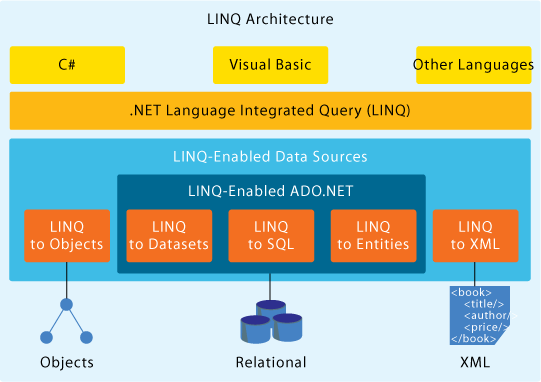
\includegraphics[width=6.4cm]{linq-arch}
\end{figure}
\end{frame}


\begin{frame}[fragile]
\frametitle{LINQ 表达式}
\begin{itemize}
\item 类似于SQL 语句的查询表达式
\end{itemize}
\begin{lstlisting}
static void Main(string[] args) {

  string[] names = {"Burke", "Connor", "Frank", 
                    "Everett", "Albert", "George", 
                    "Harris", "David" };

  IEnumerable<string> query = from s in names
                              where s.Length == 5
                              orderby s
                              select s.ToUpper();
  
  foreach(string item in query)
    Console.WriteLine(item);
}
\end{lstlisting}

\end{frame}

\begin{frame}[fragile]
\frametitle{LINQ 表达式}

\begin{lstlisting}
  var query = from s in names
              where s.Length == 5
              orderby s
              select s.ToUpper();
\end{lstlisting}
\pause

等价于如下基于方法的查询:
\begin{lstlisting}
  var query = names.Where(s => s.Length == 5)
                   .OrderBy(s => s)
                   .Select(s => s.ToUpper());
\end{lstlisting}
\pause

即使用静态类System.Linq.Enumerable 的三个扩展方法
\begin{lstlisting}
var query = Enumerable.Select(
            Enumerable.OrderBy(
            Enumerable.Where(names, 
                             s => s.Length ==5),
                             s => s),
                             s => s.ToUpper());
\end{lstlisting}
\end{frame}

\begin{frame}[fragile]
\frametitle{Enumerable的扩展方法}

\CJKindent 其中用到的是静态类System.Linq.Enumerable 中对接口 IEnumerable$<$T$>$ 的几个扩展方法

\lstset{emph={[2]Where,OrderBy,Select}}
\begin{lstlisting}
public static IEnumerable<T> Where<T>(
  this IEnumerable<T> source, Func<T, bool> predicate) {
    foreach (T item in source)
      if (predicate(item)) yield return item;
}
\end{lstlisting}
\lstset{emph={[2]Where,OrderBy,Select}}
\begin{lstlisting}
public static IOrderedEnumerable<T> OrderBy<T, K>(
    this IEnumerable<T> source, Func<T, K> keySelector)
{  ...  }
\end{lstlisting}
\lstset{emph={[2]Where,OrderBy,Select}}
\begin{lstlisting}
public static IEnumerable<R> Select<T, R>(
    this IEnumerable<T> source, Func<T, R> selector)
{  ...  }
\end{lstlisting}
\end{frame}

\begin{frame}[fragile]
\frametitle{LINQ 表达式的延迟执行}
\begin{itemize}
\item LINQ 的结果存储的是查询表达式,并没有实际的执行
\item 在对结果取值时,才触发表达式的执行,即延迟执行
\end{itemize}
\begin{lstlisting}[escapeinside='']
static void QueryOverInts()
{ int[] numbers = { 10, 20, 30, 40, 1, 2, 3, 8 };

  var subset = from i in numbers where i < 10 select i;

  foreach (var i in subset) // 'LINQ表达式被求值'
    Console.WriteLine("{0} < 10", i);

  numbers[0] = 4;
  foreach (var j in subset) // 'LINQ表达式被再次求值'
    Console.WriteLine("{0} < 10", j);
}
\end{lstlisting}
\end{frame}

\begin{frame}[fragile]
\frametitle{强制立即执行}
\begin{itemize}
\item 对查询表达式取值,触发LINQ 的执行
\item 也可以通过ToArray$<$T$>$() 或ToList$<$T$>$() 等方法
\begin{lstlisting}[escapeinside='']
static void ImmediateExecution()
{ int[] numbers = { 10, 20, 30, 40, 1, 2, 3, 8 };

  int[] toArray =       // '立即执行,并转换为数组'
             (from i in numbers 
              where i < 10 select i).ToArray<int>();

  List<int> toList =    // '立即执行,并转换为集合'
             (from i in numbers
              where i < 10 select i).ToList<int>();
}
\end{lstlisting}
\item IEnumerable$<$T$>$ 的扩展方法
\begin{itemize}
\item System.Linq.Enumerable.ToArray$<$T$>$
\item System.Linq.Enumerable.ToList$<$T$>$
\item System.Linq.Enumerable.ToDictionary$<$T,K$>$
\end{itemize}
\end{itemize}
\end{frame}


\begin{frame}[fragile]
\frametitle{LINQ 使用}
\begin{itemize}
\item \textit{namelist.txt}
\end{itemize}
\begin{lstlisting}[escapeinside='']
1       于彦秋  1090310102      0903101
2       马成龙  1090310103      0903101
3       王雪琦  1090310104      0903101
4       陈云飞  1090310105      0903101
5       张晗成  1090310106      0903101
'\dots \dots \dots ' 
\end{lstlisting}

\begin{lstlisting}[escapeinside='']
class Student{
    public int n; public string name, id, cid;
    public Student('\ldots') {
       '\ldots'
    }
    public override string ToString() {
        return string.Format(
           "序号:{0,3}  姓名:{1,4}  学号:{2}  班级:{3}",
           n, name, id, cid);}
}
\end{lstlisting}

\end{frame}


\begin{frame}[fragile]
\frametitle{LINQ 使用}

\begin{lstlisting}
static void Main(string[] args)
{
  string[] names = File.ReadAllLines(@"namelist.txt");

  var students = from x in names
                 select new Student(x.Split(' '));
  
  foreach (var x in students) Console.WriteLine(x);
}
\end{lstlisting}

\begin{lstlisting}
  Student[] students = (from x in names
             select new Student(x.Split(' '))).ToArray();
\end{lstlisting}
\end{frame}


\begin{frame}[fragile]
\frametitle{LINQ 使用 --- Basic}
\begin{itemize}
\item Drilldown
\end{itemize}
\begin{lstlisting}
var result = from x in students
             where x.name.Length == 2 && x.cid == "0903102"
             select x;
\end{lstlisting}
\begin{itemize}
\item Projection
\end{itemize}
\begin{lstlisting}
var result = from x in students
             select new {x.id, x.name};
\end{lstlisting}
\begin{itemize}
\item Filter
\end{itemize}
\begin{lstlisting}
var result = students.Where(
  (x, i) => i % int.Parse(x.id.Substring(8,2)) == 0);
\end{lstlisting}
\end{frame}

\begin{frame}[fragile]
\frametitle{LINQ 使用 --- Partition}
\begin{itemize}
\item \texttt{Take()}和\texttt{Skip()}
\begin{lstlisting}[escapeinside='']
students.Take(10)   // '前10个'
students.Skip(100)  // '除去前100个'
\end{lstlisting}

\begin{lstlisting}
(from x in students where x.cid == "0903105"
        select x.name).Take(10);
\end{lstlisting}
\item \texttt{TakeWhile()}和\texttt{SkipWhile()}

选“张某”之前的
\begin{lstlisting}
students.TakeWhile( x => x.name != "张某");
\end{lstlisting}
选15号之后的
\begin{lstlisting}
students.SkipWhile( x => x.n < 15);
\end{lstlisting}
\end{itemize}
\end{frame}




\begin{frame}[fragile]
\frametitle{LINQ 使用 --- Sort}
\begin{itemize}
\item OrderBy
\begin{lstlisting}
from x in students  orderby x.name  select x;

from x in students 
  orderby x.name.Length descending  select x;
\end{lstlisting}
\item OrderBy, ThenBy
\begin{lstlisting}
from x in students
  orderby x.cid, x.name  select x;
\end{lstlisting}
\item Reverse
\begin{lstlisting}
(from x in students
  orderby x.cid, x.name  select x).Reverse();
\end{lstlisting}
\end{itemize}
\end{frame}


\begin{frame}[fragile]
\frametitle{LINQ 使用 --- Grouping}
\begin{itemize}
\item GroupBy
\lstset{emph={group, by}}
\begin{lstlisting}
var result = from x in students group x by x.cid;

foreach (var x in result) {
    Console.WriteLine("{0}: ", x.Key);

    foreach (var y in x.ToList())
        Console.WriteLine("    {0} {1}", y.id, y.name);

}
\end{lstlisting}
\end{itemize}
\end{frame}

\begin{frame}[fragile]
\frametitle{LINQ 使用 --- Grouping}
\begin{itemize}
\item GroupBy
\lstset{emph={group, by, into}}
\begin{lstlisting}
var result = from x in students
     group x by x.name.Substring(0, 1) into y
     select new { FirstName = y.Key, Students = y };

foreach (var x in result) {
    Console.WriteLine("{0}: ", x.FirstName);

    foreach (var y in x.Students)
        Console.WriteLine("   {0} {1}", y.id, y.name);
}
\end{lstlisting}
\end{itemize}
\end{frame}


\begin{frame}[fragile]
\frametitle{LINQ 使用 --- Quantifier/Conversion}
\begin{itemize}
\item \texttt{Any, All}
\begin{lstlisting}
var result = students.Any(x => x.name == "张某");
var result = students.All(x => x.name.Length > 2);
\end{lstlisting}
\item ToArray, ToList, ToDictionary
\item OfType
\begin{lstlisting}
object[] numbers = { null, 1.0, "two", 
                     3, "four", 5, "six", 7.0 }; 
var doubles = numbers.OfType<double>(); 
foreach (var d in doubles) Console.WriteLine(d); 
// 1.0, 7.0
\end{lstlisting}
\end{itemize}
\end{frame}



\begin{frame}[fragile]
\frametitle{LINQ 使用 --- Aggregate Operators}
\begin{itemize}
\item Count
\begin{lstlisting}
students.Count();
students.Count(n => n.name.Length==3);
\end{lstlisting}
\item Sum, Min, Max, Average
\begin{lstlisting}
students.Sum(n => n.name.Length);
students.Max(n => n.name.Length);
students.Average(n => n.name.Length);
\end{lstlisting}
\end{itemize}
\end{frame}


\section{文本处理}

\begin{frame}[fragile]
\frametitle{StringBuilder 类}
可变字符串类 StringBuilder:
\begin{lstlisting}
public sealed class StringBuilder {
  public method StringBuilder();  
  public method StringBuilder(int capacity);  
  public method StringBuilder(int capacity, int maxCapacity);  
  
  public method StringBuilder(string value);  
  public method StringBuilder(string value, int capacity);  
}
\end{lstlisting}
\begin{itemize}
\item capacity --- 串的长度
\item maxCapicity --- 串的最大长度
\item 如果没有指定最大长度,会自动成倍增加
\end{itemize}
\end{frame}

\begin{frame}[fragile]
\frametitle{StringBuilder 的成员}
\begin{itemize}
\item 成员特性
\end{itemize}
\begin{lstlisting}
  public field int Capacity{set; get; } 
  public field int Length{set; get; } 
  public field int MaxCapacity{get; } 
\end{lstlisting}
\begin{itemize}
\item 成员方法
\begin{itemize}
\item Append()
\item AppendFormat()
\item Insert()
\item Replace()
\item Remove()
\end{itemize}
\end{itemize}
\end{frame}


% \begin{frame}
% \frametitle{文本的编码}

% \end{frame}

% Cookbook Regular Expressions, C# in a Nutshell

\begin{frame}
\frametitle{正则表达式}
\begin{itemize}
\setlength{\itemsep}{8pt plus 1pt}
\item 位于 System.Text.RegularExpressions 命名空间
\item 常用的类
\begin{itemize}
\setlength{\itemsep}{6pt plus 1pt}
\item Regex  --- 用于构造正则表达式对象,也有一些静态方法
\item Match, MatchCollection \\
  使用正则表达式进行匹配的结果,或结果集合
\item Group, GroupCollection \\
  正则表达式的分组匹配,即正则表达式的一部分
\item Capture, CaptureCollection \\
  分组的匹配中,由分组匹配的所有捕获
\end{itemize}
\end{itemize}
\end{frame}

\begin{frame}[fragile]
\frametitle{正则表达式示例}
\begin{lstlisting}[escapeinside='']
using System;
using System.Text.RegularExpressions;
public class List
{
  static void Main()
  {
    string s = @"<img\s+src=""(.*?)"">";
    Regex r = new Regex (s, RegexOptions.IgnoreCase) ;
    Match m = r.Match("<IMG src=\"http://abc.cn/a.jpg\">");

    for (int i=0; i<m.Groups.Count; i++)
      Console.WriteLine (m.Groups[i]);  // 'http://abc.cn/a.jpg'

    Console.ReadLine();
  }
}
\end{lstlisting}
\end{frame}

\begin{frame}[fragile]
\frametitle{特殊字符和普通字符}
\begin{tabular}{c|l}
\hline
字符                  & 说明                                               \\
\hline
\verb|.|              & 任何字符,除换行符外                               \\
\verb|* + ?|          & 前一部分的重复次数,尽可能多匹配 (\textit{greedy}) \\
\verb|\|              & 转义字符                                           \\
\verb|[|\dots\verb|]| & 字符集合,表示其中的任意字符                       \\
\verb|(|\dots\verb|)| & 分组,用于重复、引用等                             \\
\verb|{|n,m\verb|}|   & 表示匹配次数                                       \\
\verb|$|              & 行尾空串                                           \\
\verb|^|              & 行首空串                                           \\
\hline
\verb|\b|             & 单词边界上的空串                                   \\
\verb|\s|             & 匹配任何空白字符                                   \\
\verb|\w|             & 匹配任何单词                                       \\
\verb|\d|             & 匹配一个数字                                       \\
\verb|\cC|            & 匹配控制字符 Ctrl-C                               \\
\hline
\end{tabular}
\end{frame}

\begin{frame}[fragile]
\frametitle{分组及引用}
\begin{tabular}{c|l}
\hline
分组                                         & 使用方式                                       \\
\hline
\verb|(|\dots\verb|)|                        & 通过数字 \verb|\N| 引用                       \\
                                             & 例如 \verb|(\w)\s+\1|                         \\
\verb|(?<|\textit{name}\verb|>|\dots\verb|)| & 通过名字 \verb|\k<|\textit{name}\verb|>| 引用 \\
                                             & 例如 \verb|(?<word>\w)\s+\k<word>|             \\
\hline
\hline
替换方式                                     & 说明                                           \\
\hline
\verb|$|\textit{N}                           & 按组号替换                                     \\
\verb|${|\textit{name}\verb|}|               & 按组名字替换                                   \\
\hline
\end{tabular}
\medskip
\begin{lstlisting}[escapeinside='']
String ChangeDateFormat(String input)
{ // '将 mm/dd/yyyy 替换为 yyyy-mm-dd 格式'
return Regex.Replace(input,
@"\b(?<month>\d{1,2})/(?<day>\d{1,2})/(?<year>\d{2,4})\b",
"${year}-${month}-${day}");
}
\end{lstlisting}
\end{frame}

\begin{frame}[fragile]
\frametitle{正则表达式示例}
\begin{itemize}
\item 交换前两个单词
\begin{lstlisting}
string t1 = "the quick brown fox";
string p1 = @"(\S+)(\s+)(\S+)";
Regex x1 = new Regex(p1);
string r1 = x1.Replace(t1, "$3$2$1", 1);
       // "quick the brown fox"
\end{lstlisting}
\item 匹配 ``keyword = value'' 模式
\begin{lstlisting}
string t2 = "myval = 3";
string p2 = @"(\w+)\s*=\s*(.*)\s*$";
Match m2 = Regex.Match(t2, p2);
\end{lstlisting}
\end{itemize}
\end{frame}

\begin{frame}[fragile]
\frametitle{正则表达式示例}
\begin{itemize}
\item 匹配至少 40 字符的行
\begin{lstlisting}
string t3 = "aaaaaaaaaaaaaaaaaaaaaaaaaaaaaaaaaaaaaaaa"
string p3 = ".{40,}";
Match m3 = Regex.Match(t3, p3);
\end{lstlisting}
\item 替换用户名
\begin{lstlisting}
string t4 =
    @"C:\Documents and Settings\user1\Desktop";
string r4 = Regex.Replace(t4,
                          @"\\user1\\",
                          @"\\user2\\");
\end{lstlisting}
\end{itemize}
\end{frame}

% \begin{frame}[fragile]
% \frametitle{正则表达式示例}
% \begin{itemize}
% \item 查找所有字母大写的单词
% \begin{lstlisting}
% string t5 = "This IS a Test OF ALL Caps";
% string p5 = @"(\b[^\Wa-z0-9_]+\b)";
% MatchCollection mc5 = Regex.Matches(t5, p5);
% foreach (Match x in mc5)
%    Console.WriteLine(x.Groups[0].Value);
%    // IS OF ALL
% \end{lstlisting}
% \item 查找所有首字母大写的单词
% \begin{lstlisting}
% string t6 = "This is A Test of Initial Caps";
% string p6 = @"(\b[A-Z][^\WA-Z0-9_]*\b)";
% MatchCollection mc6 = Regex.Matches(t6, p6);
% \end{lstlisting}
% \end{itemize}
% \end{frame}

\begin{frame}[fragile]
\frametitle{正则表达式示例}
\begin{itemize}
\item 查找 HTML 中的URL 链接
\end{itemize}
\begin{lstlisting}[escapeinside=!!]
string t7 = @"
<html>
<a href=""http://a.b.c/news/first.htm"">first tag text</a>
<a href=""http://a.b.c/news/next.htm"">next tag text</a>
</html>
";
string p7 = @"<A[^>]*?HREF\s*=\s*[""']?"
  + @"([^'"" >]+?)[ '""]?>";
MatchCollection mc7 = 
    Regex.Matches(t7, p7, RegexOptions.Singleline
                         |RegexOptions.IgnoreCase);
foreach (Match x in mc7)
  Console.WriteLine(x.Groups[1].Value);
   // !http://a.b.c/news/first.htm!
   // !http://a.b.c/news/next.htm!
\end{lstlisting}
\end{frame}

% Local Variables:
% mode: LaTeX
% TeX-master: "part-04.tex"
% TeX-header-end: "% End-of-Header$"
% TeX-trailer-start: "% Start-of-Trailer$"
% coding: utf-8
% End:
